\documentclass[twoside]{book}

% Packages required by doxygen
\usepackage{calc}
\usepackage{doxygen}
\usepackage{graphicx}
\usepackage[utf8]{inputenc}
\usepackage{makeidx}
\usepackage{multicol}
\usepackage{multirow}
\usepackage{textcomp}
\usepackage[table]{xcolor}

% Font selection
\usepackage[T1]{fontenc}
\usepackage{mathptmx}
\usepackage[scaled=.90]{helvet}
\usepackage{courier}
\usepackage{amssymb}
\usepackage{sectsty}
\renewcommand{\familydefault}{\sfdefault}
\allsectionsfont{%
  \fontseries{bc}\selectfont%
  \color{darkgray}%
}
\renewcommand{\DoxyLabelFont}{%
  \fontseries{bc}\selectfont%
  \color{darkgray}%
}

% Page & text layout
\usepackage{geometry}
\geometry{%
  a4paper,%
  top=2.5cm,%
  bottom=2.5cm,%
  left=2.5cm,%
  right=2.5cm%
}
\tolerance=750
\hfuzz=15pt
\hbadness=750
\setlength{\emergencystretch}{15pt}
\setlength{\parindent}{0cm}
\setlength{\parskip}{0.2cm}
\makeatletter
\renewcommand{\paragraph}{%
  \@startsection{paragraph}{4}{0ex}{-1.0ex}{1.0ex}{%
    \normalfont\normalsize\bfseries\SS@parafont%
  }%
}
\renewcommand{\subparagraph}{%
  \@startsection{subparagraph}{5}{0ex}{-1.0ex}{1.0ex}{%
    \normalfont\normalsize\bfseries\SS@subparafont%
  }%
}
\makeatother

% Headers & footers
\usepackage{fancyhdr}
\pagestyle{fancyplain}
\fancyhead[LE]{\fancyplain{}{\bfseries\thepage}}
\fancyhead[CE]{\fancyplain{}{}}
\fancyhead[RE]{\fancyplain{}{\bfseries\leftmark}}
\fancyhead[LO]{\fancyplain{}{\bfseries\rightmark}}
\fancyhead[CO]{\fancyplain{}{}}
\fancyhead[RO]{\fancyplain{}{\bfseries\thepage}}
\fancyfoot[LE]{\fancyplain{}{}}
\fancyfoot[CE]{\fancyplain{}{}}
\fancyfoot[RE]{\fancyplain{}{\bfseries\scriptsize Generated on Mon Jun 5 2017 15\-:35\-:23 for Eta\-Gen by Doxygen }}
\fancyfoot[LO]{\fancyplain{}{\bfseries\scriptsize Generated on Mon Jun 5 2017 15\-:35\-:23 for Eta\-Gen by Doxygen }}
\fancyfoot[CO]{\fancyplain{}{}}
\fancyfoot[RO]{\fancyplain{}{}}
\renewcommand{\footrulewidth}{0.4pt}
\renewcommand{\chaptermark}[1]{%
  \markboth{#1}{}%
}
\renewcommand{\sectionmark}[1]{%
  \markright{\thesection\ #1}%
}

% Indices & bibliography
\usepackage{natbib}
\usepackage[titles]{tocloft}
\setcounter{tocdepth}{3}
\setcounter{secnumdepth}{5}
\makeindex

% Hyperlinks (required, but should be loaded last)
\usepackage{ifpdf}
\ifpdf
  \usepackage[pdftex,pagebackref=true]{hyperref}
\else
  \usepackage[ps2pdf,pagebackref=true]{hyperref}
\fi
\hypersetup{%
  colorlinks=true,%
  linkcolor=blue,%
  citecolor=blue,%
  unicode%
}

% Custom commands
\newcommand{\clearemptydoublepage}{%
  \newpage{\pagestyle{empty}\cleardoublepage}%
}


%===== C O N T E N T S =====

\begin{document}

% Titlepage & ToC
\hypersetup{pageanchor=false}
\pagenumbering{roman}
\begin{titlepage}
\vspace*{7cm}
\begin{center}%
{\Large Eta\-Gen }\\
\vspace*{1cm}
{\large Generated by Doxygen 1.8.5}\\
\vspace*{0.5cm}
{\small Mon Jun 5 2017 15:35:23}\\
\end{center}
\end{titlepage}
\clearemptydoublepage
\tableofcontents
\clearemptydoublepage
\pagenumbering{arabic}
\hypersetup{pageanchor=true}

%--- Begin generated contents ---
\chapter{Main Page}
\label{index}\hypertarget{index}{}An event trigger generator based on Hilbert-\/\+Huang Transform~\newline
 It is a Python module but the core library of Eta\+Gen is built in C/\+C++

\subsection*{Dependences}


\begin{DoxyItemize}
\item Numpy $>$= 1.\+10
\item Boost.\+Python $<$ 1.\+65 or $>$= 1.\+64 with Boost.\+Numpy
\end{DoxyItemize}

\#\# Install 
\begin{DoxyCode}
1 $ python setup.py install --user
\end{DoxyCode}


\subsection*{Sample U\+S\+A\+GE\+:}


\begin{DoxyItemize}
\item This shows how to generate event triggers from {\itshape data} by Eta\+Gen~\newline
 
\begin{DoxyCode}
1 >>> from etagen import etagen, kernel
2 
3 >>> h = etagen(data, fsr=1024)
4 
5 >>> h.set\_emd\_param(num\_imfs=8, num\_sifts=15, S\_number=1, emd\_size=1024, num\_seg=4,
       w\_type=kernel.SIN\_KERNEL)
6 
7 >>> h.show\_emd\_param()<br>
8 Parameters are set as follows.<br>
9 [General]<br>
10 Number of IMFs: 8<br>
11 Number of siftings:     15<br>
12 S-Number:       1<br>
13 [wSEMD settings]<br>
14 EMD size:       1024<br>
15 Number of segments:     4
16 
17 >>> h.wsemd()
18 
19 >>> h.hilbert(filter\_length=128, stride=1024)
20 
21 >>> h.get\_utriggers(snr\_th=5, stride=4*fsr, overlap=2*fsr)<br>
22 Generating triggers with 5-snr threshold in segments of length 4096, overlapping 2048 samples and skipping
       0 samples from boundaries...<br>
23 ... generated 25 trigger event(s)
24 
25 >>> h.get\_triggers(t\_tolerance=0.001, f\_tolerance=0.5, snr\_th=5.5)<br>
26 u\_snr\_th should be larger than the one used to generate triggers: assuming u\_snr\_th = 5<br>
27 Clustering triggers of u\_snr > 5 with time tolerance=0.001, frequency tolerance=0.5 and dropping clusters
       of snr < 5.5...<br>
28 total Clusters : 25 > 5.500000<br>
29 total Clusters : 12 > 5.500000<br>
30 ... generated 12 trigger cluster(s)
31 
32 >>> h.trgs[['c\_time','c\_freq','p\_time','p\_freq','npts','snr']]<br>
33 array([ (0.041015625, 297.67912076702106, 0.041015625, 297.67912076702106, 1, 5.546819634000152),<br>
34    (0.6464843749999999, 344.6262005898434, 0.646484375, 344.6262005898434, 1, 5.797973757254617),<br>
35    (1.2744140625, 260.1084208607948, 1.2744140625, 260.1084208607948, 1, 5.546288486345601),<br>
36    (1.5664062499999998, 142.61211763115602, 1.56640625, 142.61211763115602, 1, 6.513913449375204),<br>
37    (1.8193359374999998, 333.3958253278954, 1.8193359375, 333.39582532789547, 1, 6.632835601773412),<br>
38    (2.7138671875, 341.5032411355364, 2.7138671875, 341.5032411355364, 1, 6.609969624271628),<br>
39    (4.1552734375, 220.52834605967874, 4.1552734375, 220.5283460596787, 1, 5.8852032771220015),<br>
40    (4.493164062499999, 201.227897198888, 4.4931640625, 201.22789719888803, 1, 5.890950833813454),<br>
41    (5.766601562500001, 229.12911997930595, 5.7666015625, 229.12911997930595, 1, 5.557695477749056),<br>
42    (6.659179687499999, 245.8274380780258, 6.6591796875, 245.8274380780258, 1, 5.8990177018284875),<br>
43    (6.328125, 34.86349503817338, 6.328125, 34.86349503817338, 1, 5.834112766561207),<br>
44    (6.0, 67.39566743927662, 6.0, 67.39566743927662, 1, 5.9916237288573955)], <br>
45   dtype=[('c\_time', '<f8'), ('c\_freq', '<f8'), ('p\_time', '<f8'), ('p\_freq', '<f8'), ('npts', '<i8'),
       ('snr', '<f8')])
\end{DoxyCode}
 
\end{DoxyItemize}
\chapter{Namespace Index}
\section{Packages}
Here are the packages with brief descriptions (if available)\-:\begin{DoxyCompactList}
\item\contentsline{section}{\hyperlink{namespaceEtaGen}{Eta\-Gen} }{\pageref{namespaceEtaGen}}{}
\end{DoxyCompactList}

\chapter{Hierarchical Index}
\section{Class Hierarchy}
This inheritance list is sorted roughly, but not completely, alphabetically\+:\begin{DoxyCompactList}
\item etagen\begin{DoxyCompactList}
\item \contentsline{section}{python.\+\_\+wrap.\+etagen}{\pageref{classpython_1_1__wrap_1_1etagen}}{}
\end{DoxyCompactList}
\end{DoxyCompactList}

\chapter{Class Index}
\section{Class List}
Here are the classes, structs, unions and interfaces with brief descriptions\+:\begin{DoxyCompactList}
\item\contentsline{section}{\hyperlink{classpython_1_1__wrap_1_1etagen}{python.\+\_\+wrap.\+etagen} }{\pageref{classpython_1_1__wrap_1_1etagen}}{}
\end{DoxyCompactList}

\chapter{Namespace Documentation}
\hypertarget{namespaceEtaGen}{\section{Eta\-Gen Namespace Reference}
\label{namespaceEtaGen}\index{Eta\-Gen@{Eta\-Gen}}
}


\subsection{Detailed Description}
\subsection*{\hyperlink{namespaceEtaGen}{Eta\-Gen}}

An event trigger generator based on Hilbert-\/\-Huang Transform\par
 It is a Python module but the core library of \hyperlink{namespaceEtaGen}{Eta\-Gen} is built in C/\-C++

\subsubsection*{Sample U\-S\-A\-G\-E\-:}


\begin{DoxyItemize}
\item This shows how to generate event triggers from {\itshape data} by \hyperlink{namespaceEtaGen}{Eta\-Gen}\par
 $>$$>$$>$ from etagen import etagen, kernel

$>$$>$$>$ h = etagen(data, fsr=1024)

$>$$>$$>$ h.\-set\-\_\-emd\-\_\-param(num\-\_\-imfs=8, num\-\_\-sifts=15, S\-\_\-number=1, emd\-\_\-size=1024, num\-\_\-seg=4, w\-\_\-type=kernel.\-S\-I\-N\-\_\-\-K\-E\-R\-N\-E\-L)

$>$$>$$>$ h.\-show\-\_\-emd\-\_\-param()\par
 Parameters are set as follows.\par
 \mbox{[}General\mbox{]}\par
 Number of I\-M\-Fs\-: 8\par
 Number of siftings\-: 15\par
 S-\/\-Number\-: 1\par
 \mbox{[}w\-S\-E\-M\-D settings\mbox{]}\par
 E\-M\-D size\-: 1024\par
 Number of segments\-: 4

$>$$>$$>$ h.\-wsemd()

$>$$>$$>$ h.\-hilbert(filter\-\_\-length=128, stride=1024)

$>$$>$$>$ h.\-get\-\_\-utriggers(snr\-\_\-th=5, stride=4$\ast$fsr, overlap=2$\ast$fsr)\par
 Generating triggers with 5-\/snr threshold in segments of length 4096, overlapping 2048 samples and skipping 0 samples from boundaries...\par
 ... generated 25 trigger event(s)

$>$$>$$>$ h.\-get\-\_\-triggers(t\-\_\-tolerance=0.\-001, f\-\_\-tolerance=0.\-5, snr\-\_\-th=5.\-5)\par
 u\-\_\-snr\-\_\-th should be larger than the one used to generate triggers\-: assuming u\-\_\-snr\-\_\-th = 5\par
 Clustering triggers of u\-\_\-snr $>$ 5 with time tolerance=0.\-001, frequency tolerance=0.\-5 and dropping clusters of snr $<$ 5.\-5...\par
 total Clusters \-: 25 $>$ 5.\-500000\par
 total Clusters \-: 12 $>$ 5.\-500000\par
 ... generated 12 trigger cluster(s)

$>$$>$$>$ h.\-trgs\mbox{[}\mbox{[}'c\-\_\-time','c\-\_\-freq','p\-\_\-time','p\-\_\-freq','npts','snr'\mbox{]}\mbox{]}\par
 array(\mbox{[} (0.\-041015625, 297.\-67912076702106, 0.\-041015625, 297.\-67912076702106, 1, 5.\-546819634000152),\par
 (0.\-6464843749999999, 344.\-6262005898434, 0.\-646484375, 344.\-6262005898434, 1, 5.\-797973757254617),\par
 (1.\-2744140625, 260.\-1084208607948, 1.\-2744140625, 260.\-1084208607948, 1, 5.\-546288486345601),\par
 (1.\-5664062499999998, 142.\-61211763115602, 1.\-56640625, 142.\-61211763115602, 1, 6.\-513913449375204),\par
 (1.\-8193359374999998, 333.\-3958253278954, 1.\-8193359375, 333.\-39582532789547, 1, 6.\-632835601773412),\par
 (2.\-7138671875, 341.\-5032411355364, 2.\-7138671875, 341.\-5032411355364, 1, 6.\-609969624271628),\par
 (4.\-1552734375, 220.\-52834605967874, 4.\-1552734375, 220.\-5283460596787, 1, 5.\-8852032771220015),\par
 (4.\-493164062499999, 201.\-227897198888, 4.\-4931640625, 201.\-22789719888803, 1, 5.\-890950833813454),\par
 (5.\-766601562500001, 229.\-12911997930595, 5.\-7666015625, 229.\-12911997930595, 1, 5.\-557695477749056),\par
 (6.\-659179687499999, 245.\-8274380780258, 6.\-6591796875, 245.\-8274380780258, 1, 5.\-8990177018284875),\par
 (6.\-328125, 34.\-86349503817338, 6.\-328125, 34.\-86349503817338, 1, 5.\-834112766561207),\par
 (6.\-0, 67.\-39566743927662, 6.\-0, 67.\-39566743927662, 1, 5.\-9916237288573955)\mbox{]}, \par
 type=\mbox{[}('c\-\_\-time', '$<$f8'), ('c\-\_\-freq', '$<$f8'), ('p\-\_\-time', '$<$f8'), ('p\-\_\-freq', '$<$f8'), ('npts', '$<$i8'), ('snr', '$<$f8')\mbox{]}) 
\end{DoxyItemize}
\chapter{Class Documentation}
\hypertarget{classetagen}{\section{etagen Class Reference}
\label{classetagen}\index{etagen@{etagen}}
}
\subsection*{Public Member Functions}
\begin{DoxyCompactItemize}
\item 
\hypertarget{classetagen_aa580c99c23b6d9ad47e7f77838c319c4}{{\bfseries etagen} (object \&\-\_\-data=none, F\-L\-O\-A\-T \-\_\-fsr=1.\-0, F\-L\-O\-A\-T \-\_\-start\-\_\-time=0.\-0)}\label{classetagen_aa580c99c23b6d9ad47e7f77838c319c4}

\item 
void \hyperlink{classetagen_a96e7264ed9cf4f4f238fc2b645920586}{set\-\_\-data} (object \&)
\item 
\hypertarget{classetagen_a49f2c29605674eadb7f2b3c74ba6b2a8}{void {\bfseries set\-\_\-start\-\_\-time} (F\-L\-O\-A\-T \-\_\-st)}\label{classetagen_a49f2c29605674eadb7f2b3c74ba6b2a8}

\item 
\hypertarget{classetagen_aeed11ff7ed469485168426f823feb7f8}{void {\bfseries set\-\_\-fsr} (F\-L\-O\-A\-T \-\_\-fs)}\label{classetagen_aeed11ff7ed469485168426f823feb7f8}

\item 
void \hyperlink{classetagen_a910eca05e0ec09ef309761c9cd368f4c}{set\-\_\-emd\-\_\-param} (int num\-\_\-imfs=0, int num\-\_\-sifts=M\-A\-X\-\_\-\-S\-I\-F\-T, int S\-\_\-number=0, int monotonic\-\_\-spline=0, int emd\-\_\-size=2048, int num\-\_\-seg=8, int w\-\_\-type=sin\-\_\-kernel)
\item 
void \hyperlink{classetagen_a31a48ff12f1ea68d7c4d942e04bdf7e4}{show\-\_\-emd\-\_\-param} ()
\item 
void \hyperlink{classetagen_a96a89d06eac778a9804e3c8420b46c7b}{emd\-\_\-} ()
\item 
void \hyperlink{classetagen_ac3577de006721d1d9f64c7c98222be82}{wsemd\-\_\-} ()
\item 
void \hyperlink{classetagen_ad56fc2a5f5a0cf2dc20916d27b9bf64c}{set\-\_\-imf} (object \&)
\item 
void \hyperlink{classetagen_a95cd8c3d51999b0d5d8dc1ed3ed6b2bb}{set\-\_\-res} (object \&)
\item 
void \hyperlink{classetagen_a39b9c052ff247a05156ab9f0b1e8f490}{hilbert\-\_\-} (int \-\_\-filter\-\_\-len=M\-I\-N\-\_\-\-D\-H\-T\-\_\-\-F\-I\-L\-T\-E\-R\-\_\-\-L\-E\-N\-G\-T\-H, int \-\_\-stride=M\-I\-N\-\_\-\-S\-T\-R\-I\-D\-E)
\item 
void \hyperlink{classetagen_a0aa3f4df2dec5c2071712730b91153d3}{set\-\_\-hht} (object \&)
\item 
void \hyperlink{classetagen_ace17478c84198ba8eac49f4290d71b65}{set\-\_\-insa} (object \&)
\item 
void \hyperlink{classetagen_a35bc3abb1d4a49b2f6e88a389627516d}{set\-\_\-insf} (object \&)
\item 
list \hyperlink{classetagen_a49d776b1901bf1d8267e6b64792ee56f}{gen\-\_\-utrgs} (F\-L\-O\-A\-T, int, int)
\item 
numeric\-::array \hyperlink{classetagen_a83edca09f8e18a0cc618f29c1e333a13}{get\-\_\-waveform} (int)
\item 
numeric\-::array \hyperlink{classetagen_af7ace8ea08498fefd814560063e5ea39}{gen\-\_\-trgs} (numeric\-::array, F\-L\-O\-A\-T, F\-L\-O\-A\-T, F\-L\-O\-A\-T)
\end{DoxyCompactItemize}
\subsection*{Public Attributes}
\begin{DoxyCompactItemize}
\item 
\hypertarget{classetagen_a3cfb884ad14da38b25052cd1b5d8402f}{object {\bfseries data}}\label{classetagen_a3cfb884ad14da38b25052cd1b5d8402f}

\item 
\hypertarget{classetagen_a73f250a4cb0314f22349591f7b57989b}{object {\bfseries imf}}\label{classetagen_a73f250a4cb0314f22349591f7b57989b}

\item 
\hypertarget{classetagen_a08b95f16fd83fc0a7f46f68a1a2be98e}{object {\bfseries res}}\label{classetagen_a08b95f16fd83fc0a7f46f68a1a2be98e}

\item 
\hypertarget{classetagen_a42717ae51e69ab8298f349579ebb019e}{object {\bfseries hht}}\label{classetagen_a42717ae51e69ab8298f349579ebb019e}

\item 
\hypertarget{classetagen_a78dc150f9c2228ebfd864be3f37ec09e}{object {\bfseries insa}}\label{classetagen_a78dc150f9c2228ebfd864be3f37ec09e}

\item 
\hypertarget{classetagen_ab3de55a755a2603d6048fc3ec24b4b34}{object {\bfseries insf}}\label{classetagen_ab3de55a755a2603d6048fc3ec24b4b34}

\item 
\hypertarget{classetagen_a3a6debd32d5829c80fd521bb4c8f4576}{object {\bfseries utrgs}}\label{classetagen_a3a6debd32d5829c80fd521bb4c8f4576}

\item 
\hypertarget{classetagen_a1c138474ec98a0fe4a477c41b429b371}{object {\bfseries trgs}}\label{classetagen_a1c138474ec98a0fe4a477c41b429b371}

\item 
\hypertarget{classetagen_aad5224aff725e4b42df5b60a73e26bef}{int {\bfseries numberofimf}}\label{classetagen_aad5224aff725e4b42df5b60a73e26bef}

\item 
\hypertarget{classetagen_a5e2d9467f1dc2d4628279bb22d42fd47}{int {\bfseries data\-\_\-size}}\label{classetagen_a5e2d9467f1dc2d4628279bb22d42fd47}

\item 
\hypertarget{classetagen_ad53886908196e2bffbf9f254df8550b8}{F\-L\-O\-A\-T {\bfseries start\-\_\-time}}\label{classetagen_ad53886908196e2bffbf9f254df8550b8}

\item 
\hypertarget{classetagen_a596e93d478b86cac0b90943f06ff2dd6}{F\-L\-O\-A\-T {\bfseries fsr}}\label{classetagen_a596e93d478b86cac0b90943f06ff2dd6}

\end{DoxyCompactItemize}


\subsection{Detailed Description}
\hyperlink{namespaceEtaGen}{Eta\-Gen} class

U\-S\-A\-G\-E (an example)\-:\par
 h = etagen.\-etagen(data, fsr, start\-\_\-time)

arguments\-:\par
 data input data which is assumed to be whitened\par
 fsr sampling frequency\par
 start\-\_\-time start time of data in sec.

return\-:\par
 h an instance of etagen class\par


attribute stored\-:\par
 h.\-data\par
 h.\-fsr\par
 h.\-start\-\_\-time

example\-:\par
 $>$$>$$>$ import numpy as np

$>$$>$$>$ from etagen import etagen

$>$$>$$>$ h = etagen(np.\-random.\-randn(1024),32)

$>$$>$$>$ print h.\-fsr\par
 32.\-0

$>$$>$$>$ print h.\-start\-\_\-time\par
 0.\-0 

\subsection{Member Function Documentation}
\hypertarget{classetagen_a96a89d06eac778a9804e3c8420b46c7b}{\index{etagen@{etagen}!emd\-\_\-@{emd\-\_\-}}
\index{emd\-\_\-@{emd\-\_\-}!etagen@{etagen}}
\subsubsection[{emd\-\_\-}]{\setlength{\rightskip}{0pt plus 5cm}void etagen\-::emd\-\_\- (
\begin{DoxyParamCaption}
{}
\end{DoxyParamCaption}
)}}\label{classetagen_a96a89d06eac778a9804e3c8420b46c7b}
decompose self.\-data into I\-M\-Fs by E\-M\-D\par
 (parameters are set by self.\-set\-\_\-emd\-\_\-parameter) \hypertarget{classetagen_af7ace8ea08498fefd814560063e5ea39}{\index{etagen@{etagen}!gen\-\_\-trgs@{gen\-\_\-trgs}}
\index{gen\-\_\-trgs@{gen\-\_\-trgs}!etagen@{etagen}}
\subsubsection[{gen\-\_\-trgs}]{\setlength{\rightskip}{0pt plus 5cm}numeric\-::array etagen\-::gen\-\_\-trgs (
\begin{DoxyParamCaption}
\item[{numeric\-::array}]{\-\_\-utrgs, }
\item[{F\-L\-O\-A\-T}]{snr\-\_\-th, }
\item[{F\-L\-O\-A\-T}]{ttol, }
\item[{F\-L\-O\-A\-T}]{ftol}
\end{DoxyParamCaption}
)}}\label{classetagen_af7ace8ea08498fefd814560063e5ea39}
M\-E\-T\-H\-O\-D F\-O\-R T\-H\-E I\-N\-T\-E\-R\-N\-A\-L U\-S\-E \hypertarget{classetagen_a49d776b1901bf1d8267e6b64792ee56f}{\index{etagen@{etagen}!gen\-\_\-utrgs@{gen\-\_\-utrgs}}
\index{gen\-\_\-utrgs@{gen\-\_\-utrgs}!etagen@{etagen}}
\subsubsection[{gen\-\_\-utrgs}]{\setlength{\rightskip}{0pt plus 5cm}list etagen\-::gen\-\_\-utrgs (
\begin{DoxyParamCaption}
\item[{F\-L\-O\-A\-T}]{snr\-\_\-th, }
\item[{int}]{sidx, }
\item[{int}]{len}
\end{DoxyParamCaption}
)}}\label{classetagen_a49d776b1901bf1d8267e6b64792ee56f}
M\-E\-T\-H\-O\-D F\-O\-R T\-H\-E I\-N\-T\-E\-R\-N\-A\-L U\-S\-E \hypertarget{classetagen_a83edca09f8e18a0cc618f29c1e333a13}{\index{etagen@{etagen}!get\-\_\-waveform@{get\-\_\-waveform}}
\index{get\-\_\-waveform@{get\-\_\-waveform}!etagen@{etagen}}
\subsubsection[{get\-\_\-waveform}]{\setlength{\rightskip}{0pt plus 5cm}numeric\-::array etagen\-::get\-\_\-waveform (
\begin{DoxyParamCaption}
\item[{int}]{index}
\end{DoxyParamCaption}
)}}\label{classetagen_a83edca09f8e18a0cc618f29c1e333a13}
reconstruct the waveform of the {\itshape indx}-\/th trigger

arguments\-:\par
 indx the index of the trigger to reconstruct the waveform

return type\-:\par
 Numpy ndarray type \hypertarget{classetagen_a39b9c052ff247a05156ab9f0b1e8f490}{\index{etagen@{etagen}!hilbert\-\_\-@{hilbert\-\_\-}}
\index{hilbert\-\_\-@{hilbert\-\_\-}!etagen@{etagen}}
\subsubsection[{hilbert\-\_\-}]{\setlength{\rightskip}{0pt plus 5cm}void etagen\-::hilbert\-\_\- (
\begin{DoxyParamCaption}
\item[{int}]{\-\_\-filter\-\_\-len = {\ttfamily MIN\-\_\-DHT\-\_\-FILTER\-\_\-LENGTH}, }
\item[{int}]{\-\_\-stride = {\ttfamily MIN\-\_\-STRIDE}}
\end{DoxyParamCaption}
)}}\label{classetagen_a39b9c052ff247a05156ab9f0b1e8f490}
Hilbert spectral analysis

arguments\-:\par
 filter\-\_\-length length of F\-I\-R filter for D\-H\-T\par
 stride number of samples to estimate instantaneous frequency

attribute stored\-:\par
 h.\-hht Hilbert-\/transformed I\-M\-Fs\par
 h.\-insa instantaneous amplitudes of I\-M\-Fs\par
 h.\-insf instantaneous frequnecies of I\-M\-Fs \hypertarget{classetagen_a96e7264ed9cf4f4f238fc2b645920586}{\index{etagen@{etagen}!set\-\_\-data@{set\-\_\-data}}
\index{set\-\_\-data@{set\-\_\-data}!etagen@{etagen}}
\subsubsection[{set\-\_\-data}]{\setlength{\rightskip}{0pt plus 5cm}void etagen\-::set\-\_\-data (
\begin{DoxyParamCaption}
\item[{object \&}]{a}
\end{DoxyParamCaption}
)}}\label{classetagen_a96e7264ed9cf4f4f238fc2b645920586}
(re)set the input data

example\-:\par
 $>$$>$$>$ import numpy as np

$>$$>$$>$ from etagen import etagen

$>$$>$$>$ h = etagen(np.\-random.\-randn(1024))

$>$$>$$>$ print h.\-data.\-shape\par
 (1024,)

$>$$>$$>$ h.\-set\-\_\-data(np.\-random.\-randn(32))

$>$$>$$>$ print h.\-data.\-shape\par
 (32,) \hypertarget{classetagen_a910eca05e0ec09ef309761c9cd368f4c}{\index{etagen@{etagen}!set\-\_\-emd\-\_\-param@{set\-\_\-emd\-\_\-param}}
\index{set\-\_\-emd\-\_\-param@{set\-\_\-emd\-\_\-param}!etagen@{etagen}}
\subsubsection[{set\-\_\-emd\-\_\-param}]{\setlength{\rightskip}{0pt plus 5cm}void etagen\-::set\-\_\-emd\-\_\-param (
\begin{DoxyParamCaption}
\item[{int}]{num\-\_\-imfs = {\ttfamily 0}, }
\item[{int}]{num\-\_\-sifts = {\ttfamily MAX\-\_\-SIFT}, }
\item[{int}]{S\-\_\-number = {\ttfamily 0}, }
\item[{int}]{monotonic\-\_\-spline = {\ttfamily 0}, }
\item[{int}]{emd\-\_\-size = {\ttfamily 2048}, }
\item[{int}]{num\-\_\-seg = {\ttfamily 8}, }
\item[{int}]{w\-\_\-type = {\ttfamily sin\-\_\-kernel}}
\end{DoxyParamCaption}
)}}\label{classetagen_a910eca05e0ec09ef309761c9cd368f4c}
(re)set the parameters for (w\-S)E\-M\-D

arguments\-:\par
 num\-\_\-imfs number of I\-M\-Fs to be obtained\par
 num\-\_\-sifts maximum number of siftings to obtain each I\-M\-F\par
 S\-\_\-number criterion to stop sifting,\par
 (number of extrema) -\/ (number of zero-\/crossings) $<$= S\-\_\-number\par
 emd\-\_\-size (for w\-S\-E\-M\-D) number of data samples in each E\-M\-D segments\par
 num\-\_\-seg (for w\-S\-E\-M\-D) number of segments to average out the I\-M\-Fs\par
 w\-\_\-type (for w\-S\-E\-M\-D) type of weighting kernel\par
 (see docstring of etagen.\-kernel)\par
 \hypertarget{classetagen_a0aa3f4df2dec5c2071712730b91153d3}{\index{etagen@{etagen}!set\-\_\-hht@{set\-\_\-hht}}
\index{set\-\_\-hht@{set\-\_\-hht}!etagen@{etagen}}
\subsubsection[{set\-\_\-hht}]{\setlength{\rightskip}{0pt plus 5cm}void etagen\-::set\-\_\-hht (
\begin{DoxyParamCaption}
\item[{object \&}]{a}
\end{DoxyParamCaption}
)}}\label{classetagen_a0aa3f4df2dec5c2071712730b91153d3}
(re)set the Hilbert-\/transformed I\-M\-Fs \hypertarget{classetagen_ad56fc2a5f5a0cf2dc20916d27b9bf64c}{\index{etagen@{etagen}!set\-\_\-imf@{set\-\_\-imf}}
\index{set\-\_\-imf@{set\-\_\-imf}!etagen@{etagen}}
\subsubsection[{set\-\_\-imf}]{\setlength{\rightskip}{0pt plus 5cm}void etagen\-::set\-\_\-imf (
\begin{DoxyParamCaption}
\item[{object \&}]{a}
\end{DoxyParamCaption}
)}}\label{classetagen_ad56fc2a5f5a0cf2dc20916d27b9bf64c}
set or replace I\-M\-Fs \hypertarget{classetagen_ace17478c84198ba8eac49f4290d71b65}{\index{etagen@{etagen}!set\-\_\-insa@{set\-\_\-insa}}
\index{set\-\_\-insa@{set\-\_\-insa}!etagen@{etagen}}
\subsubsection[{set\-\_\-insa}]{\setlength{\rightskip}{0pt plus 5cm}void etagen\-::set\-\_\-insa (
\begin{DoxyParamCaption}
\item[{object \&}]{a}
\end{DoxyParamCaption}
)}}\label{classetagen_ace17478c84198ba8eac49f4290d71b65}
(re)set the instantaneous amplitudes of I\-M\-Fs \hypertarget{classetagen_a35bc3abb1d4a49b2f6e88a389627516d}{\index{etagen@{etagen}!set\-\_\-insf@{set\-\_\-insf}}
\index{set\-\_\-insf@{set\-\_\-insf}!etagen@{etagen}}
\subsubsection[{set\-\_\-insf}]{\setlength{\rightskip}{0pt plus 5cm}void etagen\-::set\-\_\-insf (
\begin{DoxyParamCaption}
\item[{object \&}]{a}
\end{DoxyParamCaption}
)}}\label{classetagen_a35bc3abb1d4a49b2f6e88a389627516d}
(re)set the instantaneous frequencies of I\-M\-Fs \hypertarget{classetagen_a95cd8c3d51999b0d5d8dc1ed3ed6b2bb}{\index{etagen@{etagen}!set\-\_\-res@{set\-\_\-res}}
\index{set\-\_\-res@{set\-\_\-res}!etagen@{etagen}}
\subsubsection[{set\-\_\-res}]{\setlength{\rightskip}{0pt plus 5cm}void etagen\-::set\-\_\-res (
\begin{DoxyParamCaption}
\item[{object \&}]{a}
\end{DoxyParamCaption}
)}}\label{classetagen_a95cd8c3d51999b0d5d8dc1ed3ed6b2bb}
(re)set the residual \hypertarget{classetagen_a31a48ff12f1ea68d7c4d942e04bdf7e4}{\index{etagen@{etagen}!show\-\_\-emd\-\_\-param@{show\-\_\-emd\-\_\-param}}
\index{show\-\_\-emd\-\_\-param@{show\-\_\-emd\-\_\-param}!etagen@{etagen}}
\subsubsection[{show\-\_\-emd\-\_\-param}]{\setlength{\rightskip}{0pt plus 5cm}void etagen\-::show\-\_\-emd\-\_\-param (
\begin{DoxyParamCaption}
{}
\end{DoxyParamCaption}
)}}\label{classetagen_a31a48ff12f1ea68d7c4d942e04bdf7e4}
show the parameters for (w\-S)E\-M\-D \hypertarget{classetagen_ac3577de006721d1d9f64c7c98222be82}{\index{etagen@{etagen}!wsemd\-\_\-@{wsemd\-\_\-}}
\index{wsemd\-\_\-@{wsemd\-\_\-}!etagen@{etagen}}
\subsubsection[{wsemd\-\_\-}]{\setlength{\rightskip}{0pt plus 5cm}void etagen\-::wsemd\-\_\- (
\begin{DoxyParamCaption}
{}
\end{DoxyParamCaption}
)}}\label{classetagen_ac3577de006721d1d9f64c7c98222be82}
decompose self.\-data into I\-M\-Fs by w\-S\-E\-M\-D\par
 (parameters are set by self.\-set\-\_\-emd\-\_\-parameter) 

The documentation for this class was generated from the following file\-:\begin{DoxyCompactItemize}
\item 
etagen.\-cpp\end{DoxyCompactItemize}

\hypertarget{classpython_1_1__wrap_1_1etagen}{\section{python.\-\_\-wrap.\-etagen Class Reference}
\label{classpython_1_1__wrap_1_1etagen}\index{python.\-\_\-wrap.\-etagen@{python.\-\_\-wrap.\-etagen}}
}
Inheritance diagram for python.\-\_\-wrap.\-etagen\-:\begin{figure}[H]
\begin{center}
\leavevmode
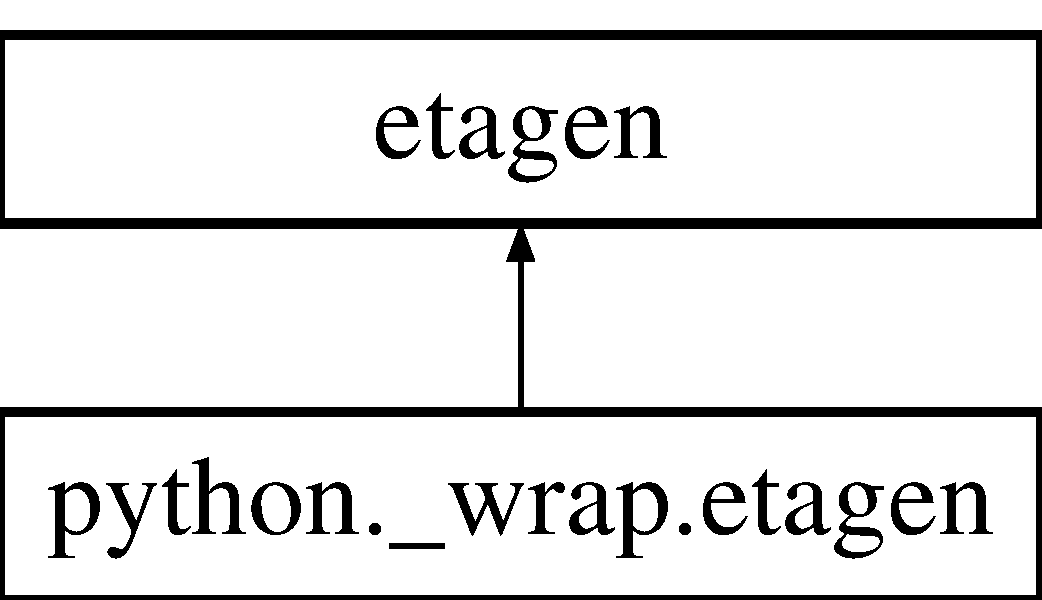
\includegraphics[height=2.000000cm]{classpython_1_1__wrap_1_1etagen}
\end{center}
\end{figure}
\subsection*{Public Member Functions}
\begin{DoxyCompactItemize}
\item 
def \hyperlink{classpython_1_1__wrap_1_1etagen_a27945aeb4059ba3b81e38fff12ea5424}{get\-\_\-utriggers}
\item 
def \hyperlink{classpython_1_1__wrap_1_1etagen_a73614979353f43ac4bfc923bce68d2cd}{get\-\_\-utriggers\-\_\-from\-\_\-file}
\item 
def \hyperlink{classpython_1_1__wrap_1_1etagen_a6f332e2242c9bb8b87dc593f17542873}{get\-\_\-triggers}
\item 
def \hyperlink{classpython_1_1__wrap_1_1etagen_add5689086be59da228ee79535f19aa8a}{get\-\_\-triggers\-\_\-from\-\_\-file}
\item 
def \hyperlink{classpython_1_1__wrap_1_1etagen_adba206932fb4791a553a36d147c43bd8}{copy}
\item 
def \hyperlink{classpython_1_1__wrap_1_1etagen_a5393c44d9e6a8754dda3a3835f66cebb}{plot\-\_\-tfd}
\item 
def \hyperlink{classpython_1_1__wrap_1_1etagen_aa8188f4111faefd7df20a40e7a233afd}{plot\-\_\-trgs}
\end{DoxyCompactItemize}
\subsection*{Public Attributes}
\begin{DoxyCompactItemize}
\item 
\hypertarget{classpython_1_1__wrap_1_1etagen_ade022a3ddd38334c6a1c4666e4b791e2}{{\bfseries min\-\_\-snr}}\label{classpython_1_1__wrap_1_1etagen_ade022a3ddd38334c6a1c4666e4b791e2}

\item 
\hypertarget{classpython_1_1__wrap_1_1etagen_a64f39feb7baa26e4a048455eea79672f}{{\bfseries std}}\label{classpython_1_1__wrap_1_1etagen_a64f39feb7baa26e4a048455eea79672f}

\item 
\hypertarget{classpython_1_1__wrap_1_1etagen_a8d72e02eb9ef5898d29e07a4f8bf35f7}{{\bfseries trg\-\_\-skip}}\label{classpython_1_1__wrap_1_1etagen_a8d72e02eb9ef5898d29e07a4f8bf35f7}

\item 
\hypertarget{classpython_1_1__wrap_1_1etagen_aedc63ca3e4633696c1d1432ae5af65e7}{{\bfseries trg\-\_\-stride}}\label{classpython_1_1__wrap_1_1etagen_aedc63ca3e4633696c1d1432ae5af65e7}

\item 
\hypertarget{classpython_1_1__wrap_1_1etagen_abef066c8bcca998720ed758824cc27c0}{{\bfseries trg\-\_\-overlap}}\label{classpython_1_1__wrap_1_1etagen_abef066c8bcca998720ed758824cc27c0}

\item 
\hypertarget{classpython_1_1__wrap_1_1etagen_ab9a3023653e8bc4fa767509c1f0cbb18}{{\bfseries utrgs}}\label{classpython_1_1__wrap_1_1etagen_ab9a3023653e8bc4fa767509c1f0cbb18}

\item 
\hypertarget{classpython_1_1__wrap_1_1etagen_afdf0a29439d61d5226ba044da470edf0}{{\bfseries u\-\_\-snr\-\_\-threshold}}\label{classpython_1_1__wrap_1_1etagen_afdf0a29439d61d5226ba044da470edf0}

\item 
\hypertarget{classpython_1_1__wrap_1_1etagen_a7f8badecd73f47578c62974a0e74080d}{{\bfseries snr\-\_\-threshold}}\label{classpython_1_1__wrap_1_1etagen_a7f8badecd73f47578c62974a0e74080d}

\item 
\hypertarget{classpython_1_1__wrap_1_1etagen_a3f69ad9121ced6715a6a3e52de40536e}{{\bfseries trgs}}\label{classpython_1_1__wrap_1_1etagen_a3f69ad9121ced6715a6a3e52de40536e}

\end{DoxyCompactItemize}
\subsection*{Static Public Attributes}
\begin{DoxyCompactItemize}
\item 
\hypertarget{classpython_1_1__wrap_1_1etagen_abd7912f308ef9623da9dfcea0e8a1c95}{list {\bfseries utrg\-\_\-dtype} = \mbox{[}('imf\-\_\-idx',int), ('s\-\_\-time',float), ('e\-\_\-time',float), ('p\-\_\-time',float), ('p\-\_\-amp',float), ('p\-\_\-freq',float), ('f\-\_\-min',float), ('f\-\_\-max',float), ('snr',float)\mbox{]}}\label{classpython_1_1__wrap_1_1etagen_abd7912f308ef9623da9dfcea0e8a1c95}

\item 
\hypertarget{classpython_1_1__wrap_1_1etagen_a9e04218bd2d74e12cc0a91f5f8fd0bc1}{list {\bfseries trg\-\_\-dtype} = \mbox{[}('s\-\_\-time',float), ('e\-\_\-time',float), ('c\-\_\-time',float), ('c\-\_\-freq',float), ('c\-\_\-energy',float), ('p\-\_\-time',float), ('p\-\_\-freq',float), ('p\-\_\-amp',float), ('p\-\_\-imf\-\_\-idx',int), ('p\-\_\-snr',float), ('f\-\_\-min',float), ('f\-\_\-max',float), ('npts',int), ('snr\-\_\-rss',float), ('snr',float)\mbox{]}}\label{classpython_1_1__wrap_1_1etagen_a9e04218bd2d74e12cc0a91f5f8fd0bc1}

\end{DoxyCompactItemize}


\subsection{Member Function Documentation}
\hypertarget{classpython_1_1__wrap_1_1etagen_adba206932fb4791a553a36d147c43bd8}{\index{python\-::\-\_\-wrap\-::etagen@{python\-::\-\_\-wrap\-::etagen}!copy@{copy}}
\index{copy@{copy}!python::_wrap::etagen@{python\-::\-\_\-wrap\-::etagen}}
\subsubsection[{copy}]{\setlength{\rightskip}{0pt plus 5cm}def python.\-\_\-wrap.\-etagen.\-copy (
\begin{DoxyParamCaption}
\item[{}]{self, }
\item[{}]{start = {\ttfamily None}, }
\item[{}]{end = {\ttfamily None}}
\end{DoxyParamCaption}
)}}\label{classpython_1_1__wrap_1_1etagen_adba206932fb4791a553a36d147c43bd8}
\begin{DoxyVerb}hhtout = self.copy(start=None, end=None):

Copy HHT instance [from *start* second to *end* second, if specified]
*start*/*end* should be greater than self.start_time

Input parameters:

    start       start time to copy the data
    end     end time to copy the data

Output parameters:

    hhtout      copied HHT instance
\end{DoxyVerb}
 \hypertarget{classpython_1_1__wrap_1_1etagen_a6f332e2242c9bb8b87dc593f17542873}{\index{python\-::\-\_\-wrap\-::etagen@{python\-::\-\_\-wrap\-::etagen}!get\-\_\-triggers@{get\-\_\-triggers}}
\index{get\-\_\-triggers@{get\-\_\-triggers}!python::_wrap::etagen@{python\-::\-\_\-wrap\-::etagen}}
\subsubsection[{get\-\_\-triggers}]{\setlength{\rightskip}{0pt plus 5cm}def python.\-\_\-wrap.\-etagen.\-get\-\_\-triggers (
\begin{DoxyParamCaption}
\item[{}]{self, }
\item[{}]{snr\-\_\-th = {\ttfamily 10}, }
\item[{}]{t\-\_\-tolerance = {\ttfamily 0.}, }
\item[{}]{f\-\_\-tolerance = {\ttfamily 0.}, }
\item[{}]{u\-\_\-snr\-\_\-th = {\ttfamily 3}}
\end{DoxyParamCaption}
)}}\label{classpython_1_1__wrap_1_1etagen_a6f332e2242c9bb8b87dc593f17542873}
\begin{DoxyVerb}self.get_triggers(maxDist=2):

Cluster trigger events generated by self.get_utriggers().

Required item:

    self.utrgs  triggers generated by self.get_utriggers()

Input parameters:

    maxDist     maximum distance to cluster tiggers. Default is 2.
    unit_time   unit time for distance. Default is 0.01(=10ms).
    u_snr_th    A threshold parameter for each trigger event. Default is 3.
    snr_th  A threshold parameter for a cluster of triggers.
    Default is 10.
    
Output:

    self.utrgs  The trigger information generated if not calculated before.
    The information is [IMF index, start time, end time,
    peak time, peak amplitude, peak frequency, snr].
    self.trgs   The trigger cluster information generated.
\end{DoxyVerb}
 \hypertarget{classpython_1_1__wrap_1_1etagen_add5689086be59da228ee79535f19aa8a}{\index{python\-::\-\_\-wrap\-::etagen@{python\-::\-\_\-wrap\-::etagen}!get\-\_\-triggers\-\_\-from\-\_\-file@{get\-\_\-triggers\-\_\-from\-\_\-file}}
\index{get\-\_\-triggers\-\_\-from\-\_\-file@{get\-\_\-triggers\-\_\-from\-\_\-file}!python::_wrap::etagen@{python\-::\-\_\-wrap\-::etagen}}
\subsubsection[{get\-\_\-triggers\-\_\-from\-\_\-file}]{\setlength{\rightskip}{0pt plus 5cm}def python.\-\_\-wrap.\-etagen.\-get\-\_\-triggers\-\_\-from\-\_\-file (
\begin{DoxyParamCaption}
\item[{}]{self, }
\item[{}]{trg\-\_\-file, }
\item[{}]{kwargs}
\end{DoxyParamCaption}
)}}\label{classpython_1_1__wrap_1_1etagen_add5689086be59da228ee79535f19aa8a}
\begin{DoxyVerb}self.get_triggers_from_file(trg_file, **kwargs):

Read clustered trigger events from file

Input parameters:

    trg_file    Filename that contains clustered trigger informations
    in ASCII format
    **kwargs    kwargs for numpy.loadtxt or numpy.fromfile
    
Output:

    self.trgs   The trigger cluster information generated.
\end{DoxyVerb}
 \hypertarget{classpython_1_1__wrap_1_1etagen_a27945aeb4059ba3b81e38fff12ea5424}{\index{python\-::\-\_\-wrap\-::etagen@{python\-::\-\_\-wrap\-::etagen}!get\-\_\-utriggers@{get\-\_\-utriggers}}
\index{get\-\_\-utriggers@{get\-\_\-utriggers}!python::_wrap::etagen@{python\-::\-\_\-wrap\-::etagen}}
\subsubsection[{get\-\_\-utriggers}]{\setlength{\rightskip}{0pt plus 5cm}def python.\-\_\-wrap.\-etagen.\-get\-\_\-utriggers (
\begin{DoxyParamCaption}
\item[{}]{self, }
\item[{}]{snr\-\_\-th = {\ttfamily 3}, }
\item[{}]{stride = {\ttfamily 0}, }
\item[{}]{overlap = {\ttfamily 0}, }
\item[{}]{skip = {\ttfamily 0}}
\end{DoxyParamCaption}
)}}\label{classpython_1_1__wrap_1_1etagen_a27945aeb4059ba3b81e38fff12ea5424}
\begin{DoxyVerb}self.get_utriggers(snr_th=3, stride=0, overlap=0, skip=0):

Generate triggers, provided that Intrinsic Mode Functions(IMFs) are
obtained before self.get_utriggers() is called.

Required item:

    self.imfs   IMFs obtained by self.get_imfs()

Input parameters:

    s       A threshold parameter. Default is 3.
    stride      The length of segment in which triggers are generated.
    overlap     The length of overlap of two neighboring segments.
    skip        The length of skipped samples at boundaries of IMFs.
    
Output:

    self.utrgs  The trigger information generated.
    The information is [IMF index, start time, end time,
    peak time, peak amplitude, peak frequency, snr].
\end{DoxyVerb}
 \hypertarget{classpython_1_1__wrap_1_1etagen_a73614979353f43ac4bfc923bce68d2cd}{\index{python\-::\-\_\-wrap\-::etagen@{python\-::\-\_\-wrap\-::etagen}!get\-\_\-utriggers\-\_\-from\-\_\-file@{get\-\_\-utriggers\-\_\-from\-\_\-file}}
\index{get\-\_\-utriggers\-\_\-from\-\_\-file@{get\-\_\-utriggers\-\_\-from\-\_\-file}!python::_wrap::etagen@{python\-::\-\_\-wrap\-::etagen}}
\subsubsection[{get\-\_\-utriggers\-\_\-from\-\_\-file}]{\setlength{\rightskip}{0pt plus 5cm}def python.\-\_\-wrap.\-etagen.\-get\-\_\-utriggers\-\_\-from\-\_\-file (
\begin{DoxyParamCaption}
\item[{}]{self, }
\item[{}]{trg\-\_\-file, }
\item[{}]{kwargs}
\end{DoxyParamCaption}
)}}\label{classpython_1_1__wrap_1_1etagen_a73614979353f43ac4bfc923bce68d2cd}
\begin{DoxyVerb}self.get_utriggers_from_file(trg_file, **kwargs):

Read triggers from file

Input parameters:

    trg_file    Filename that contains trigger informations in ASCII format
    **kwargs    kwargs for numpy.loadtxt or numpy.fromfile
    
Output:

    self.utrgs  The trigger information generated.
    The information is [IMF index, start time, end time,
    peak time, peak amplitude, peak frequency, snr].
\end{DoxyVerb}
 \hypertarget{classpython_1_1__wrap_1_1etagen_a5393c44d9e6a8754dda3a3835f66cebb}{\index{python\-::\-\_\-wrap\-::etagen@{python\-::\-\_\-wrap\-::etagen}!plot\-\_\-tfd@{plot\-\_\-tfd}}
\index{plot\-\_\-tfd@{plot\-\_\-tfd}!python::_wrap::etagen@{python\-::\-\_\-wrap\-::etagen}}
\subsubsection[{plot\-\_\-tfd}]{\setlength{\rightskip}{0pt plus 5cm}def python.\-\_\-wrap.\-etagen.\-plot\-\_\-tfd (
\begin{DoxyParamCaption}
\item[{}]{self, }
\item[{}]{indices = {\ttfamily None}, }
\item[{}]{kwargs}
\end{DoxyParamCaption}
)}}\label{classpython_1_1__wrap_1_1etagen_a5393c44d9e6a8754dda3a3835f66cebb}
\begin{DoxyVerb}self.plot_tfd(indices=None, **kwargs):

Plot time-frequency-distribution (TFD)

Input parameters:

    indices     List of indices of IMFs used for plotting TFD
    All IMFs will be used by default.
    **kwargs    kwargs for matplotlib.pyplot.scatter
\end{DoxyVerb}
 \hypertarget{classpython_1_1__wrap_1_1etagen_aa8188f4111faefd7df20a40e7a233afd}{\index{python\-::\-\_\-wrap\-::etagen@{python\-::\-\_\-wrap\-::etagen}!plot\-\_\-trgs@{plot\-\_\-trgs}}
\index{plot\-\_\-trgs@{plot\-\_\-trgs}!python::_wrap::etagen@{python\-::\-\_\-wrap\-::etagen}}
\subsubsection[{plot\-\_\-trgs}]{\setlength{\rightskip}{0pt plus 5cm}def python.\-\_\-wrap.\-etagen.\-plot\-\_\-trgs (
\begin{DoxyParamCaption}
\item[{}]{self, }
\item[{}]{indices = {\ttfamily None}, }
\item[{}]{clustered = {\ttfamily True}, }
\item[{}]{scale = {\ttfamily True}, }
\item[{}]{kwargs}
\end{DoxyParamCaption}
)}}\label{classpython_1_1__wrap_1_1etagen_aa8188f4111faefd7df20a40e7a233afd}
\begin{DoxyVerb}self.plot_trgs(indices=None, **kwargs):

Plot trigger-gram

Input parameters:

    indices     List of indices of triggers used for plotting trigger-gram
    All triggers will be used by default.
    **kwargs    kwargs for matplotlib.pyplot.scatter
\end{DoxyVerb}
 

The documentation for this class was generated from the following file\-:\begin{DoxyCompactItemize}
\item 
\-\_\-wrap.\-py\end{DoxyCompactItemize}

%--- End generated contents ---

% Index
\newpage
\phantomsection
\addcontentsline{toc}{part}{Index}
\printindex

\end{document}
